\begin{frame}[label=current]
 \frametitle{Euclidean Distance in Coordinates}

   Points $A(x_A,y_A,z_A)$ and $B(x_B,y_B,z_B)$:
   %
\begin{figure}[h]
  \psfrag{O}{$O$}
  \psfrag{A}{$A$} 
  \psfrag{B}{$B(x_B, y_B, z_B)$}  
  \psfrag{C}{$C(x_B, y_B, z_A)$}    
  \psfrag{x}{$y$} 
  \psfrag{y}{$x$} 
  \psfrag{z}{$z$}     
  \psfrag{dx}{$y_B - y_A$}
  \psfrag{dy}{$x_B - x_A$}
  \psfrag{dz}{$z_B - z_A$}  
  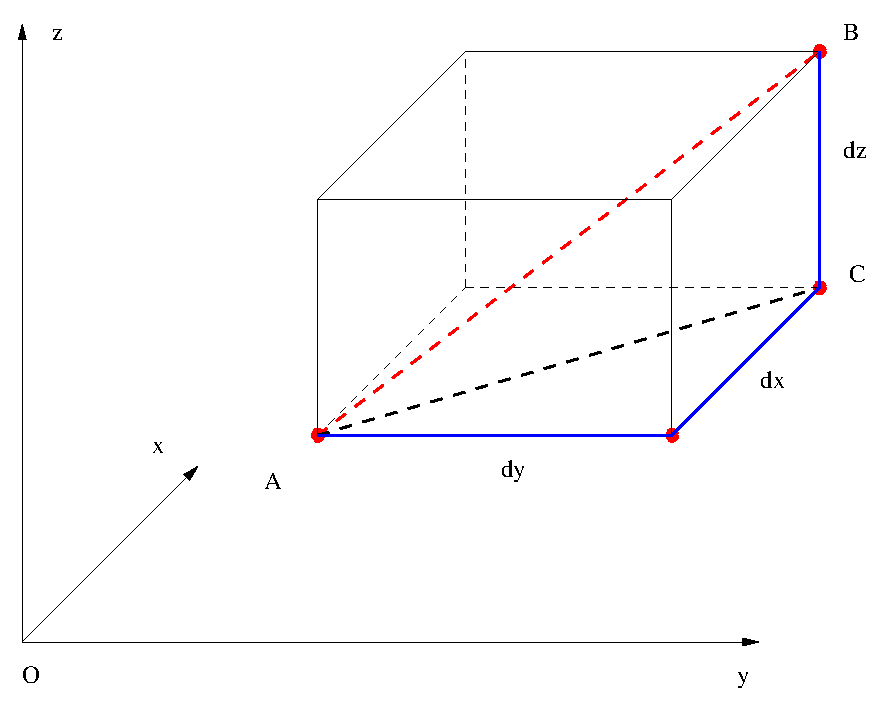
\includegraphics[height=2in]{./images/euclidean_distance.eps}
  %\caption{Euclidean distance}
  %\label{fig:euclidean_distance}
\end{figure}
%
$$d(A,B) = |AB| = \sqrt{(x_B-x_A)^2+(y_B-y_A)^2+(z_B-z_A)^2}$$
%
Example: $P(3,1,2)$ and $Q(1,2,3)$:\pause
%
$$D(P,Q) = \sqrt{(1-3)^2+(2-1)^2+(3-2)^2} = \sqrt{6}\; .$$

\end{frame}